\section{System overview}\label{sec:overview}

\subsection{Design principles}

\begin{enumerate}
  \item \textbf{Wrap, don't fork.} AgentPassport sits \emph{around} AX: in front of its API, inside its runner contract, and on the network path out of the sandbox. AX keeps doing what it does well.
  \item \textbf{The agent is untrusted.} Everything inside the sandbox, including the agent's own code, may be compromised. Therefore no signing key, no long-lived credential and no policy decision lives inside the sandbox.
  \item \textbf{Chokepoints over good behaviour.} We do not ask the agent to sign its requests or to respect its limits. We place a gateway on the only way out and enforce limits there.
  \item \textbf{Every action traces back to a human.} A passport always names a principal; sub-task passports name their parent; the chain ends at a person who logged in.
  \item \textbf{Trust is continuous.} A passport is short-lived (hours, not months), revocable at any moment, and its holder's score is re-evaluated with every event.
  \item \textbf{Verifiable by anyone.} Relying parties need only public keys and standard libraries to verify requests.
\end{enumerate}

\subsection{Architecture}

Figure~\ref{fig:arch} (printed in landscape after this section's text) shows all components. Purple boxes are ours, grey boxes are AX and Agent Substrate (unchanged), green boxes are the outside world.



\textbf{Walkthrough of the numbered arrows:}

\begin{enumerate}[label=\protect\circled{\arabic*},leftmargin=2em]
  \item The principal logs in with the university OIDC provider (browser or device-code flow from the terminal) and obtains an ID token.
  \item The principal runs \code{ax apply -f task.yaml}. The CLI is configured with \code{--server} (or \code{AX\_SERVER}) pointing to our \comp{admission proxy}, and the ID token is sent as gRPC metadata. The CLI sends the task as an \code{UpdateTask} call, which AX uses both to create and to update tasks.
  \item The admission proxy checks the task against the \comp{policy store} and asks the \comp{passport authority} (PA) to issue a passport. The PA also creates a fresh signing key pair for the task.
  \item The proxy forwards the (slightly modified) \code{UpdateTask} call to the real \code{ax-server}. The modification: the image is switched to our KYA runner image if needed, and environment variables pointing at the egress gateway are added.
  \item AX and Agent Substrate create the sandbox as usual. The \comp{KYA runner} (our build of \code{ax-task-runner}) starts, prepares the workspace, and launches the agent with all traffic routed through the gateway.
  \item Every outbound HTTP request of the agent reaches the \comp{egress gateway}.
  \item The gateway checks the allowlist, attaches the passport, signs the request with the task's key, and forwards it to the relying party, where the \comp{KYA verifier} middleware checks it before the application sees it. Calls to LLM and MCP endpoints in the visa are forwarded (and metered) too.
  \item The verifier fetches public keys and revocation status from the PA (and caches them).
  \item The gateway, the runner and the verifier's decisions feed events to the \comp{trust observer}.
  \item If a task's trust score falls below the suspend threshold, the observer calls \code{SuspendTask} on \code{ax-server} and asks the PA to revoke the passport.
\end{enumerate}

Every component also writes its security-relevant events to the \comp{audit ledger}; the \comp{console} reads from the ledger, the observer and the PA.

\subsection{End-to-end sequence}

Figure~\ref{fig:seq} (landscape, after Figure~\ref{fig:arch}) shows the same flow over time, split into the three phases of a task's life: \emph{launch}, \emph{act} and \emph{watch}. In practice the ``act'' and ``watch'' phases repeat for every request the agent makes.



\begin{landscape}
\begin{figure}[p]
  \centering
  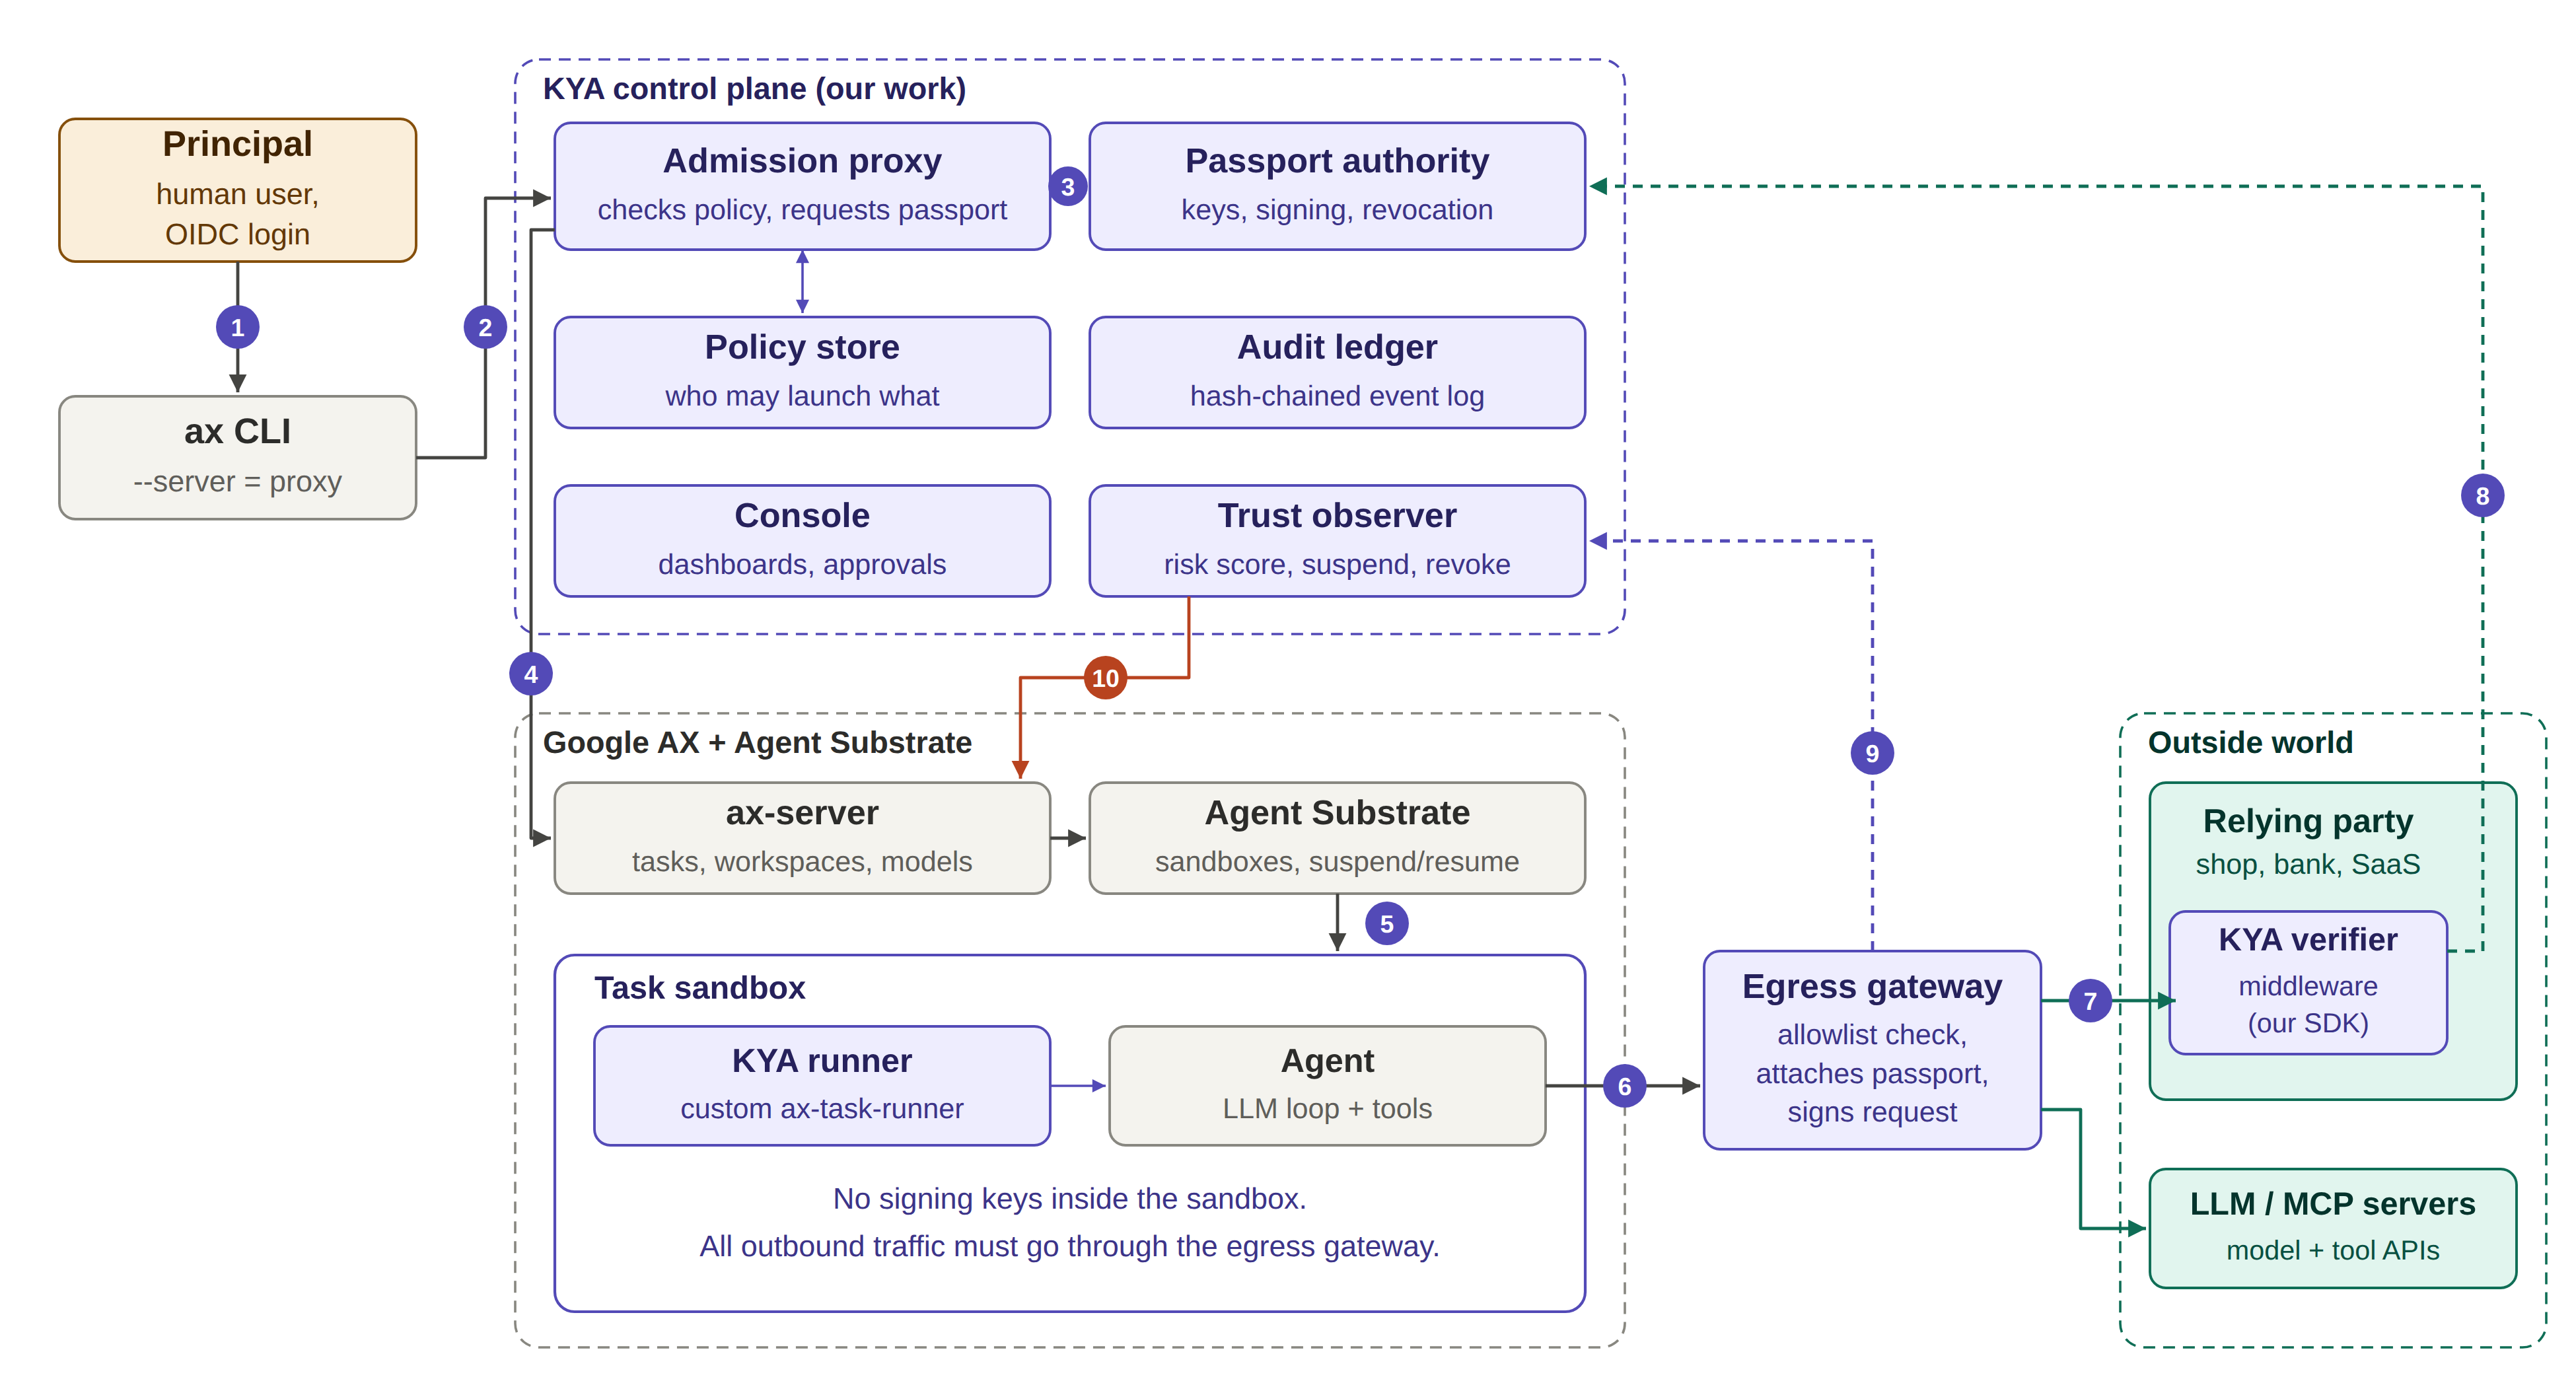
\includegraphics[width=\linewidth,height=0.86\textheight,keepaspectratio]{system_architecture.png}
  \caption{AgentPassport architecture. Purple: our components; grey: AX and Agent Substrate (unchanged); green: the outside world. Numbers refer to the walkthrough in Section~\ref{sec:overview}.}
  \label{fig:arch}
\end{figure}
\end{landscape}

\begin{landscape}
\begin{figure}[p]
  \centering
  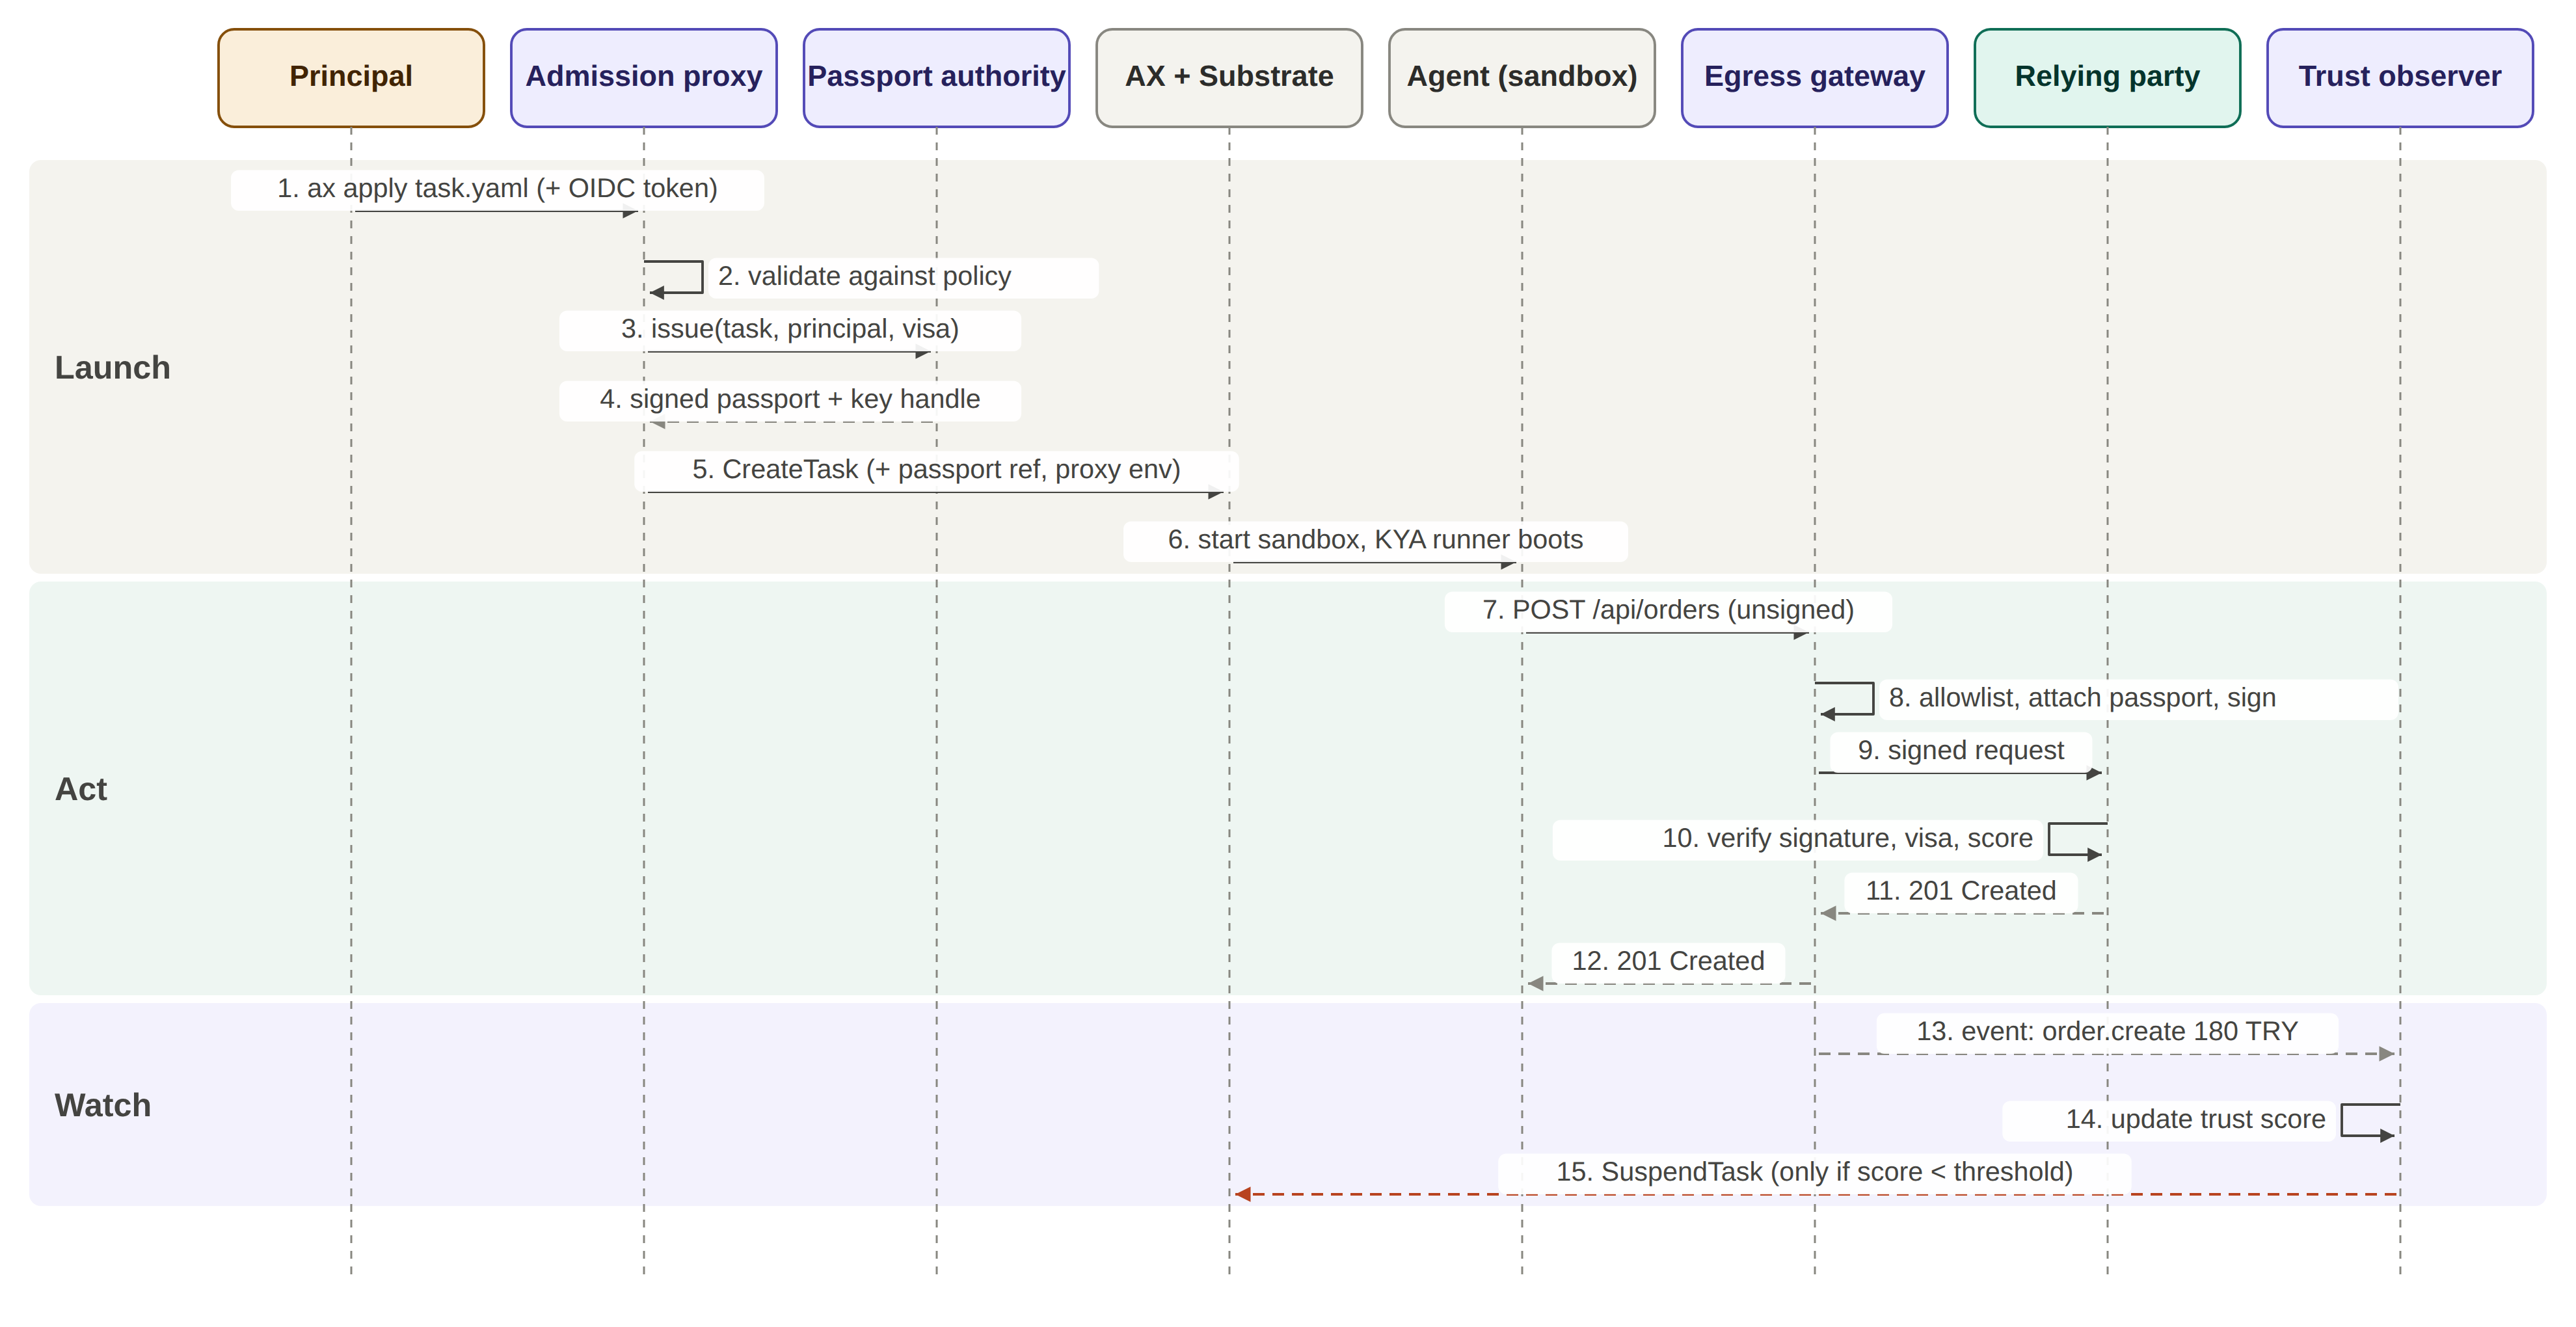
\includegraphics[width=\linewidth,height=0.86\textheight,keepaspectratio]{sequence.png}
  \caption{Sequence of a task's life with AgentPassport. Dashed arrows are responses or asynchronous events. Step~15 only happens if the trust score falls below the threshold.}
  \label{fig:seq}
\end{figure}
\end{landscape}

\subsection{How AgentPassport attaches to AX}\label{sec:seams}

Because AX is young and changing, the integration points are kept narrow and explicit. If one of them changes upstream, only one adapter has to be updated.

\begin{center}
\small
\begin{tabularx}{\linewidth}{@{}L{3.2cm}L{4.5cm}Y@{}}
\toprule
\textbf{Seam} & \textbf{AX feature used} & \textbf{What we do there}\\
\midrule
API front door & \code{ax --server} or \code{AX\_SERVER}; gRPC service \code{ax.v1alpha1.AX} (\code{UpdateTask}; \code{Update}/\code{Delete} for gateways, workspaces, models) & Admission proxy implements the same gRPC service, authenticates, checks policy, forwards to \code{ax-server}. Changes to gateways, workspaces and models are restricted by policy (Section~\ref{sec:admission}).\\
Control-plane access & Kubernetes NetworkPolicy on \code{ax-server} & Only the admission proxy and \code{ax-controller} can reach \code{ax-server}, so the proxy cannot be bypassed.\\
Inside the sandbox & Runner contract; \codeurl{github.com/google/ax/runner} package; \code{spec.image} & KYA runner = default runner + proxy environment + trust bundle + event reporting.\\
Network path out & Substrate egress controls, Kubernetes NetworkPolicy & Only the egress gateway is reachable from sandboxes.\\
Emergency brake & \code{SuspendTask} / \code{DeleteTask} RPCs & Trust observer suspends tasks automatically.\\
Discovery & \code{GetTask}, \code{WatchTask} RPCs & Observer and console follow task lifecycle.\\
\bottomrule
\end{tabularx}
\end{center}

\begin{warnbox}[Assumption to verify early]
Forcing \emph{all} sandbox egress through the gateway depends on configuring Agent Substrate's egress controls (or a Kubernetes NetworkPolicy on the worker pods). In the first weeks we will verify exactly how this can be configured in our installation. As a fallback for the prototype, the KYA runner sets \code{HTTP\_PROXY}/\code{HTTPS\_PROXY}, which is enough for cooperative agents but not for a malicious one; the evaluation will state clearly which mode was used.
\end{warnbox}
